
\section{Specification \& Design}\label{process}

\subsection{User Requirements Survey Design}

\subsubsection{Ethics Form}
Before beginning the process of gathering user requirements, an ethics form was drafted and completed to ensure that the research follows ethical guidelines. This Ethics form included a summary of all progress to date, included how participants were recruited, what information participants received about the study and what they were expected to do, and how user data was stored and processed. 

\subsubsection{Recruitment}
To recruit participants for the study, personal contacts in this demographic (women between the ages of 30 and 60) were invited and the supervisor for this project utilised professional and colleague email contacts and distribution lists to identify and invite women to participate. 

\subsubsection{Survey Design}
In preparation for building the product, participants were asked to complete a questionnaire via Microsoft Forms and so a User Requirements survey was designed. In preparation, research was conducted through books on women’s experiences during perimenopause, including works by Kat Muir\cite{Muir2022} and Davina McCall\cite{McCall2022}, as well as reviewing research papers on health-tracking applications and a review of existing apps on the market to assess current solutions. Privacy emerged as a significant concern, with many apps engaging in surveillance capitalism and selling user data, often without informing the user or by misleading the user\cite{Gilman_2021}\cite{FTC2021}. Hackers are lured to health data such as that stored by symptom tracking apps because on the black market, a person's medical data sells for 50 times what credit card information sells for\cite{Rosato2020}. This meant that the surveys myst include oppertunities for the uers to give their opinions on privacy and their priorities in a tracking app.

The first page of all online surveys conducted during the study contained the consent form with text stated that by completing the survey, they were implying consent to take part in that phase. This User Requirements questionnaire contained questions regarding the users age, menopause stage, symptoms they experience, if they track their symptoms/periods, how, and the frequency of tracking. It also included questions to see if they share tracking data with their healthcare provider and if it was helpful. Along with tracking challenges, triggers, menopause medication or treatment. The final questions included open ended questions about tracking frustrations, helpful aspects of tracking, challenges in understanding/identifying patterns, reminder preferences, and insights/features a user might like to see in a tracking app. 

\subsubsection{App feedback Survey Design} 
User interviews were also conducted to refine the design based on feedback. 


%% Susan:
%% I'm not convinced that the background section is the right place 
%% to evaluate whether to use Kanban or Scrum.  
%% Unless you've already been given explicit feedback to include it there, 
%% I would consider moving your evalution to this section instead, 
%% to have evaluation and informed decision in one place.  
%% 
\subsection{Methodology}
Following research on the different available software lifecycle approach softwares and methods available, Kanban boards were chosen as they are easy to maintain for one person, help with workflow, and have been proven to work in a student setting as mentioned prior. GitLab Issue boards were selected as the platform to host the Kanban as each issue card can be linked to branches within repositories to keep track of which tasks and changes are for which branches to improve organisation. Three labels: Code, Writing and research, and Critical, were also added to signify the type of task for each issue card. The Kanban board included four sections, one for each label and one for closed tasks. Gitlab would automatically sort each task into the relevent section based on its labels. The board was updated regularly to reflect the current status of each task, and tasks were moved from one section to another as they were completed. This resulted in tasks that were easy to prioritise, order, track, and complete on time. See Figure \ref{figure:kanban-board} for the Kanban board.

\begin{figure}[h!!]
  \begin{center}
    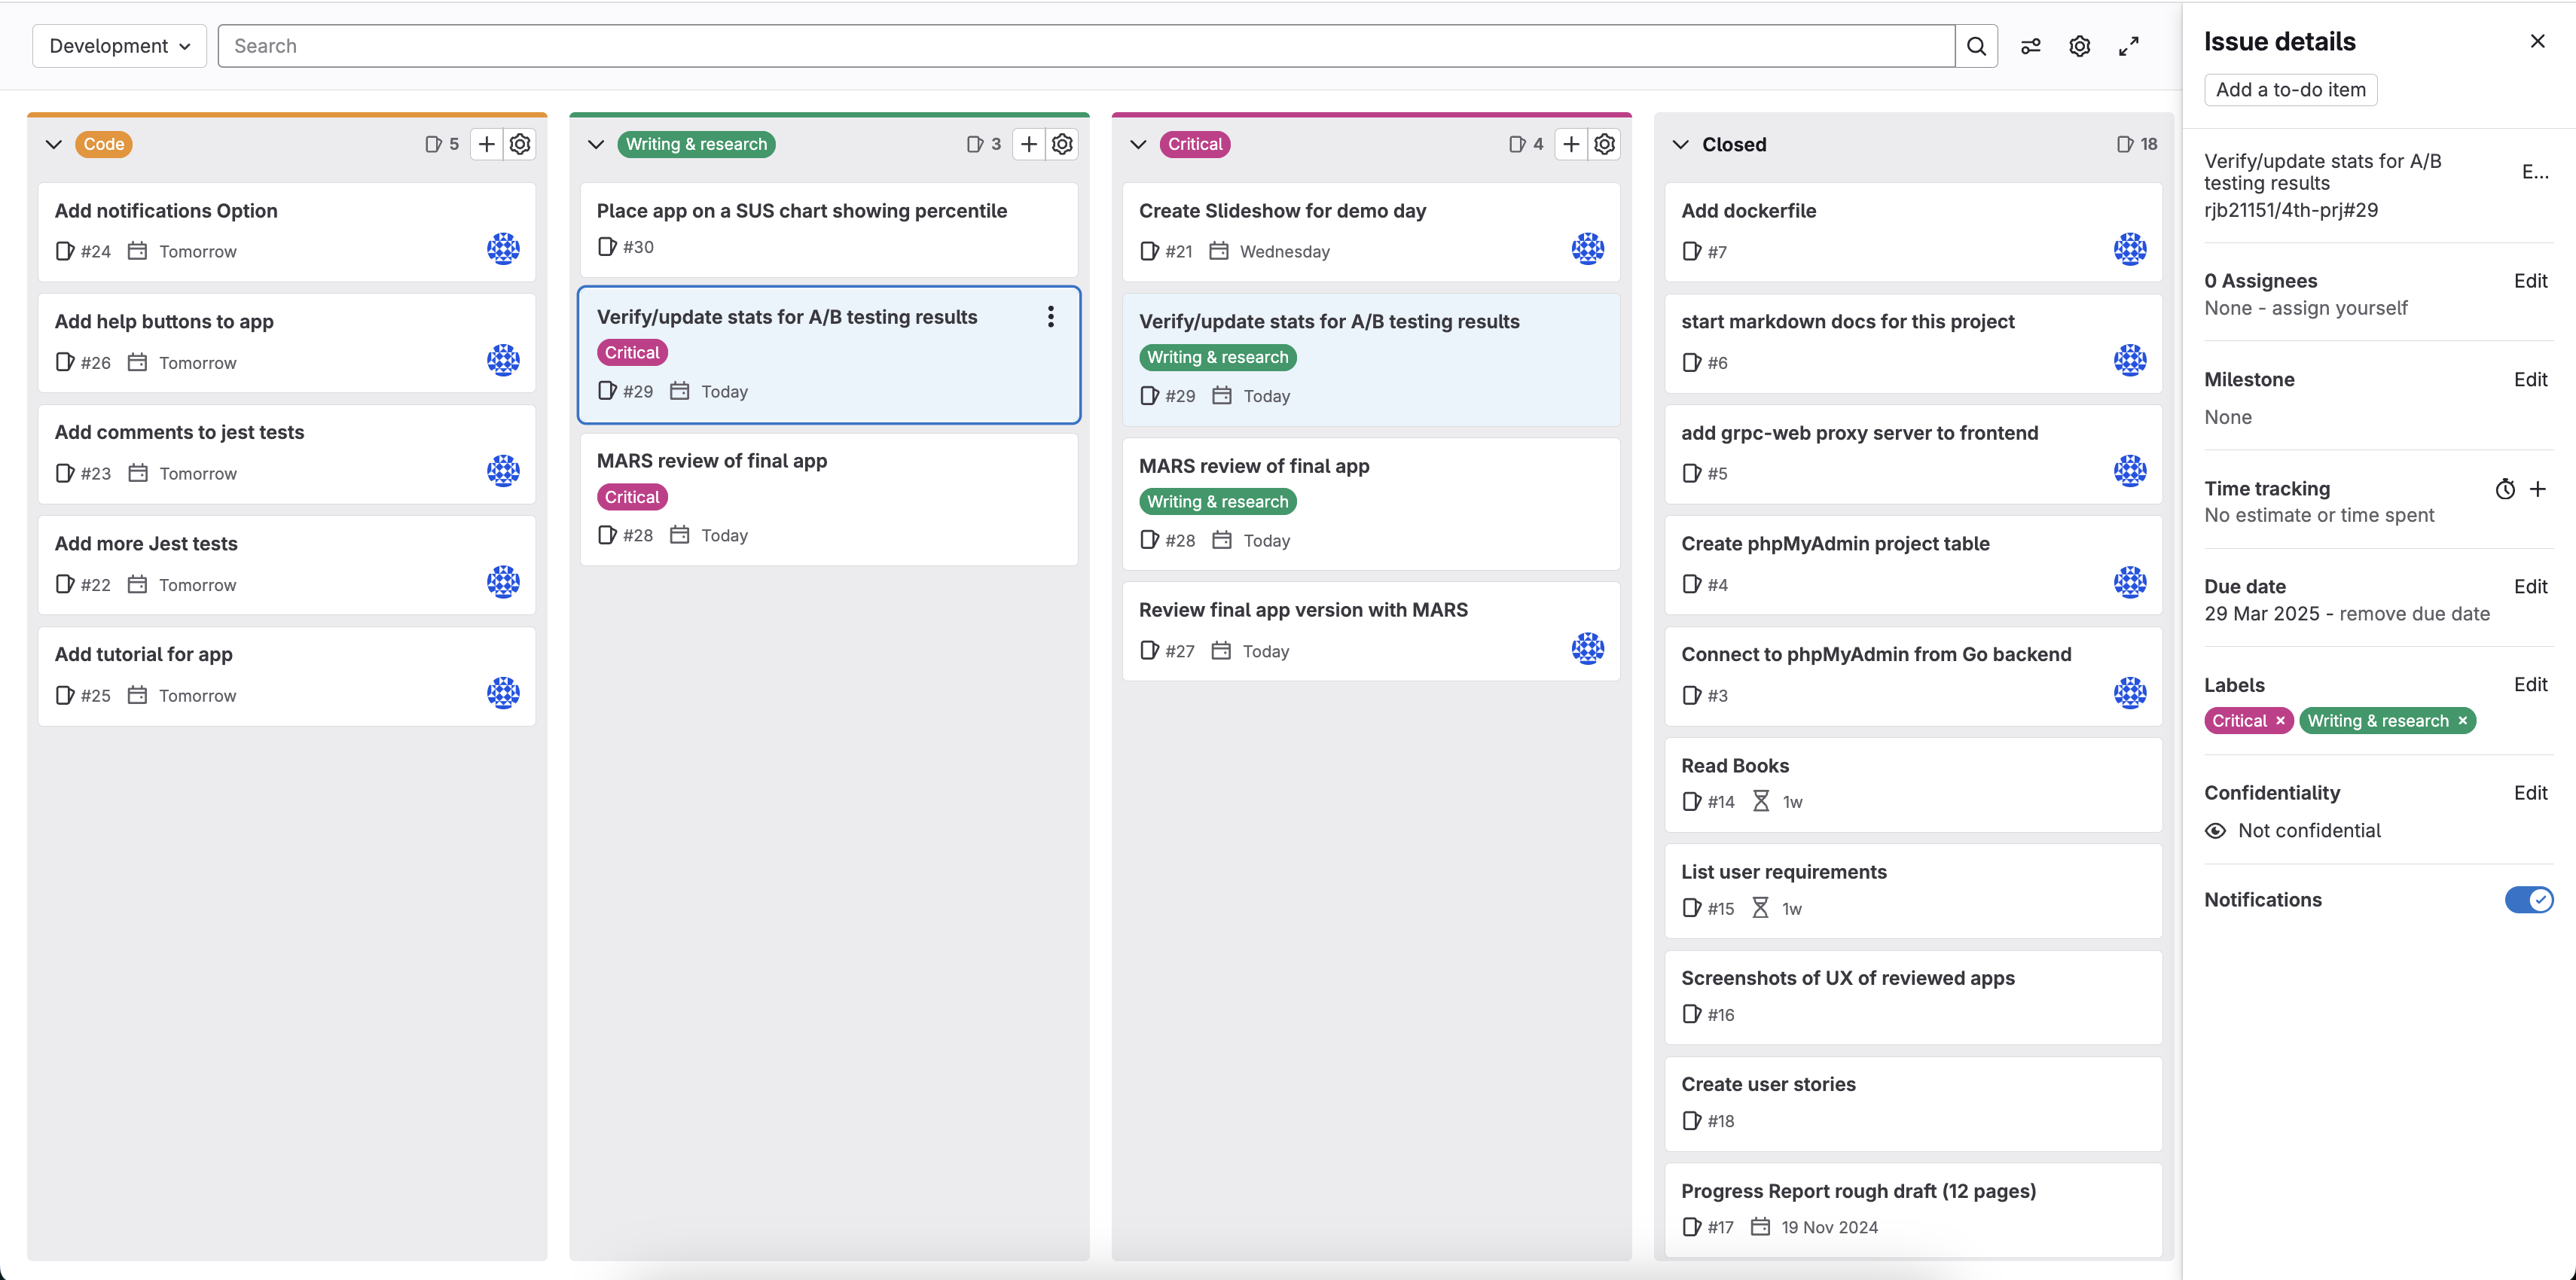
\includegraphics[scale=0.25]{Kanban.png}
    \caption{Kanban board on GitLab.}
    \label{figure:kanban-board}
  \end{center}
\end{figure}

After around a month of progress, a network diagram was made to find the critical path in order to correctly prioritise work. Once a list of the main activities was made, the dependencies of each activity were identified and the time it would take to complete each activity was estimated. The critical path was then identified by finding the path through the network diagram with a float or leeway of zero. The critical path is the sequence of activities that must be completed on time for the project to be completed on schedule. The critical path is important because it helps to identify which activities are most important for the success of the project and which activities can be delayed without affecting the overall project timeline. See Figure \ref{figure:network-diagram} for the network diagram. The critical path activities are highlighted in red. From the network diagram, it was concluded that writing the report and obtaining feedback was the most important aspect of this project and should be prioritised over other tasks. The network diagram also helped to identify potential bottlenecks in the project timeline and allowed for better planning and scheduling of tasks.

\begin{figure}[h!!]
  \begin{center}
    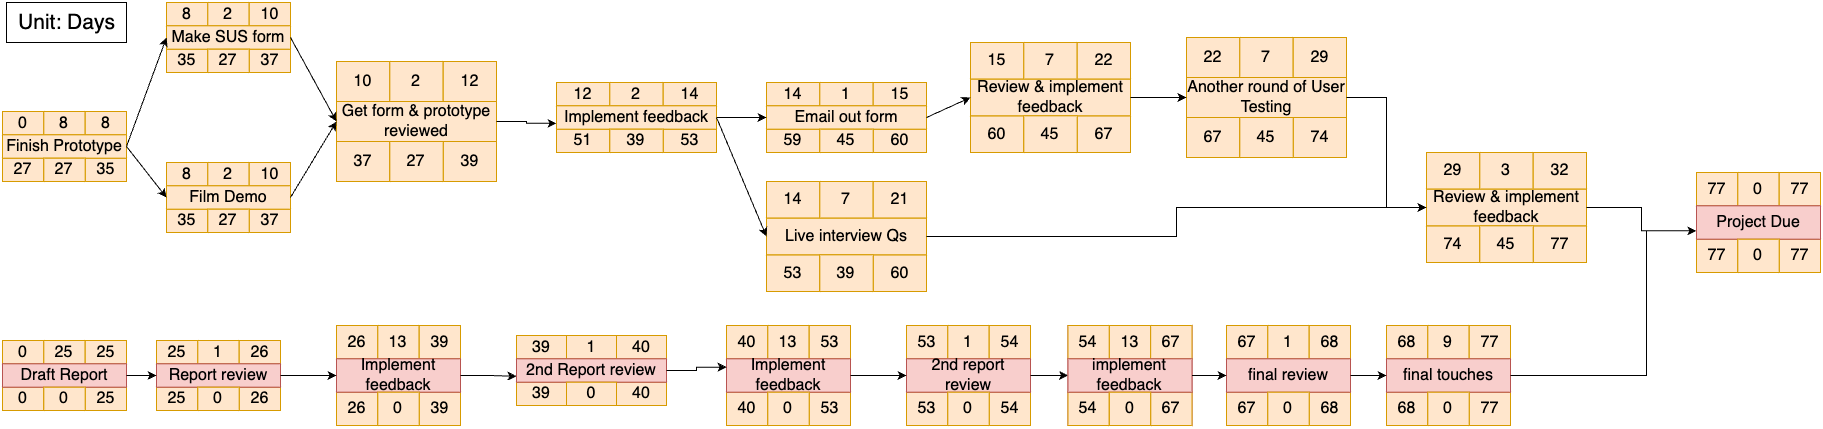
\includegraphics[scale=0.2]{NetworkDiagram.drawio.png}
    \caption{Network Diagram showing critical path.}
    \label{figure:network-diagram}
  \end{center}
\end{figure}
 
\subsection{Analysis}
Given many peri-menopausal women are not receiving support from the government education system or their doctors\cite{Aljumah2023}\cite{MenopauseSupport2021}\cite{UCL2023}, additional resources and tools must be provided to help them navigate this stage of life. With the rise of technology, several tools are now available to allow women to track their peri-menopausal symptoms. However, these tools are often not user-friendly, do not provide enough educational information, or are not privacy-focused. The issue around privacy is especially concerning as many apps are selling user data to third parties without user knowledge and consent, and in today's political climate this can result in the incarceration of the user in some parts of the US\cite{Kelly2023}. Since there are no apps that provide a comprehensive solution to these problems, the goal of this project is to create a user-friendly, educational, and privacy-focused peri-menopausal symptom tracking app.

\subsection{Requirements}

\subsubsection{Functional Requirements}
This App's functional requirements were prioritized based on user needs and the project goal. Essential functional requirements impacting usability such as being able to navigate to a screen were prioritised over design and content details. The following functional requirements were identified:

\begin{itemize}
      \item Users must be able to log their period start and end dates to track cycle and period length.
      \item Users must be able to log their peri-menopausal symptoms and their severity daily to track changes over time.
      \item Users must be able to edit or delete logged symptoms and period data at any time.
      \item The app must store all user data locally using AsyncStorage on the users device, ensuring no data is stored on external servers.
      \item The app must include a calendar view where users can see logged symptoms and period data over time.
      \item The app must provide an option to reset user data to align with privacy-focused design principles
      \item The app must provide graph-based visualizations showing symptom frequency and period heaviness trends over time.
      \item The app must calculate and display the most common symptom based on user entries.
      \item The app must provide cycle length insights based on logged period data.
      \item The app must calculate average period length based on tracked cycles.
      \item Users must be able to access an Analysis Tab summarizing trends.
      \item The app must feature a Learn Page with information on perimenopause and related topics.
      \item Users must be able to access external links to trusted resources for more detailed information.
      \item The app must follow EU accessibility standards, including text scaling, color contrast, and screen reader compatibility.
      \item The app must support multiple languages to accommodate diverse users.
      \item Users must be able to enable or disable notifications/reminders for period tracking or symptom logging.
      \item The app must work fully offline, allowing users to track symptoms and view their data without an internet connection.
      \item The app must not crash or freeze during normal usage.
\end{itemize}

\subsubsection{Non-Functional Requirements}
\begin{itemize}
  \item The app should be easy to use and navigate, with a clean and simple design.
  \item The app home page should load within 3 seconds.
  \item All data visualization such as graphs, calendar, and analysis charts should render in under 2 seconds.
  \item The app should allow easy localization to support multiple languages.
  \item The UI should offer a dark mode and high-contrast mode to improve readability for all users.
  \item All text elements must support dynamic font resizing based on user preferences.
  \item The app should look the same for various screen sizes, including tablets and smaller phones.
  \item The app must be designed with easy language switching to support multiple languages in the future.
  \item The app should maintain consistent navigation and UI patterns across all features to reduce confusion.
\end{itemize}

\subsection{Design}

\subsubsection{Interface Design}
At the beginning of the design process, low fidelity wireframes were created using Figma (See Figure \ref{figure:figma-1}).

\begin{figure}[h!!]
  \begin{center}
    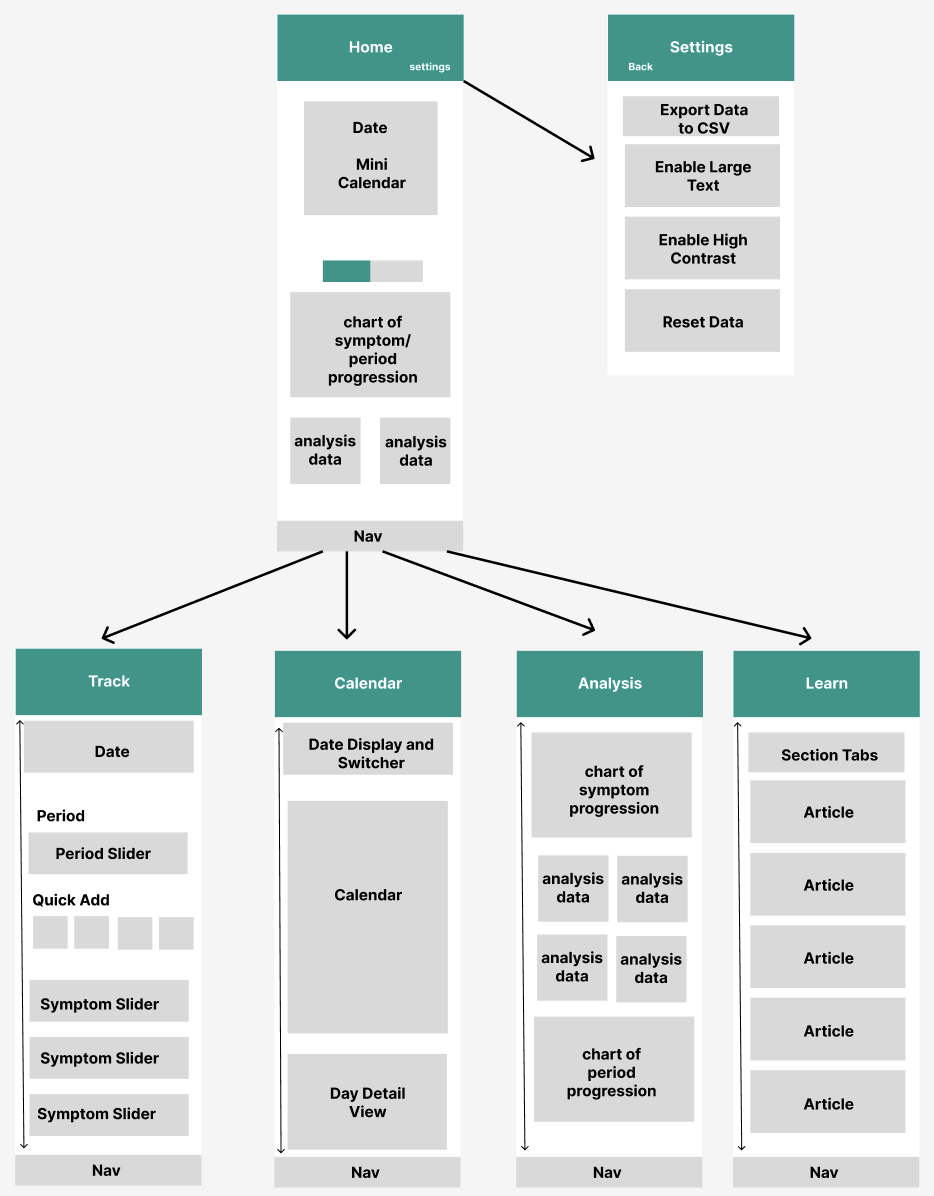
\includegraphics[scale=0.7]{Figma-1.png}
    \caption{Wireframe of App on Figma.}
    \label{figure:figma-1}
  \end{center}
\end{figure}

The colour scheme was chosen to be relaxing and calming  through the use of blue and green tones. The app was designed to be user-friendly and intuitive, with a focus on simplicity and ease of use. The design was also created with the goal of making it easy for users to navigate the app and find the information they need, as well as be responsive and work well on different screen sizes, including tablets and smaller phones.  

The design was then fleshed out into a more detailed figma design. See Figure \ref{figure:figma-2}.

\begin{figure}[h!!]
  \begin{center}
    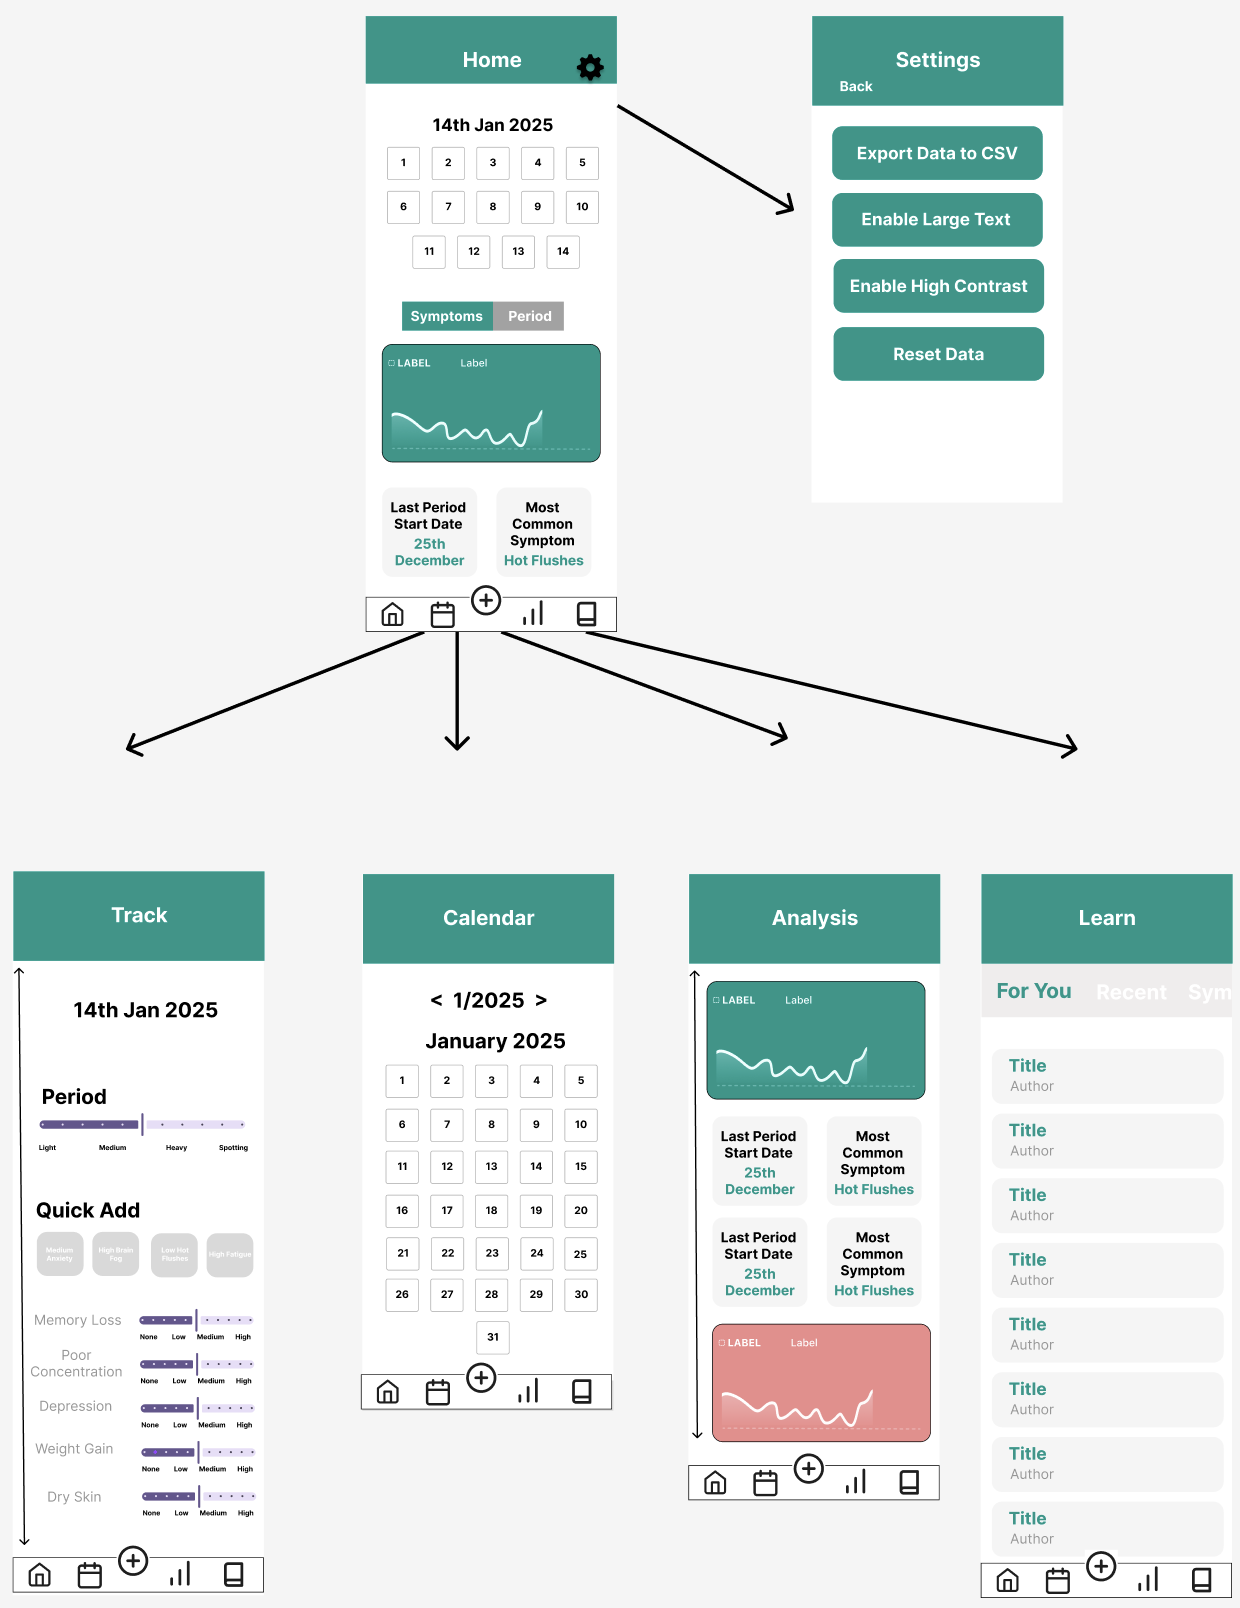
\includegraphics[scale=0.6]{Figma-2.png}
    \caption{Deatiled Draft of App on Figma.}
    \label{figure:figma-2}
  \end{center}
\end{figure}

The final design as seen in figure\ref{figure:app} was created with a focus on simplicity and ease of use. The app was designed to be user-friendly and intuitive, with a clean and simple design. The final color scheme was chosen to be calming and easy on the eyes, with a focus on blues and greens. Feedback from user evaluations was incorporated into the design to ensure that it met the needs of the target audience. Some user feedback that was implemented includes adding days of the week to the mini calendar in the home page, making the track button in the nav bar larger and a different color to make it more visible, ability to refresh the home page, and ability to track by clicking a day in the calendar. 

\begin{figure}[h!!]
  \begin{center}
    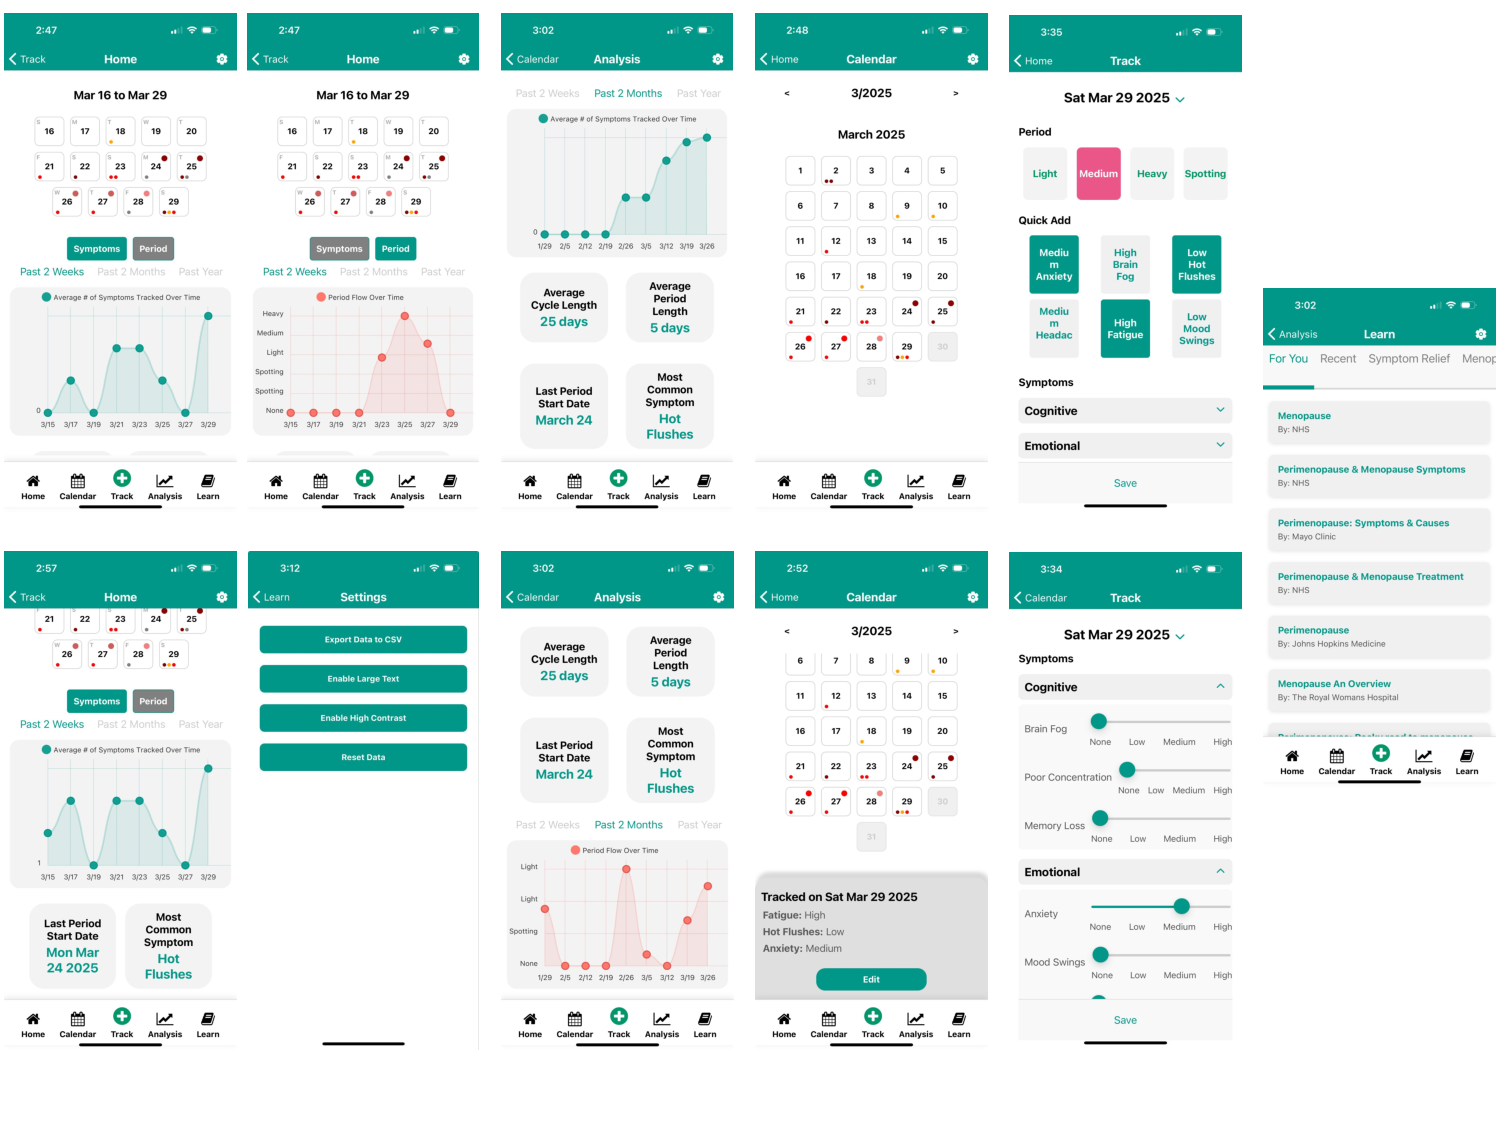
\includegraphics[scale=0.6]{app.pdf}
    \caption{Final React Native App Design.}
    \label{figure:app}
  \end{center}
\end{figure}


The app was then compared to the EU WAG 2.1 accessibility standards and adjusted to be accessible to all users, with large text and color contrast options in the settings. Figure \ref{figure:app-Accessible} shows the app in dark mode with high contrast and large text mode enabled.
 
\begin{figure}[h!!]
  \begin{center}
    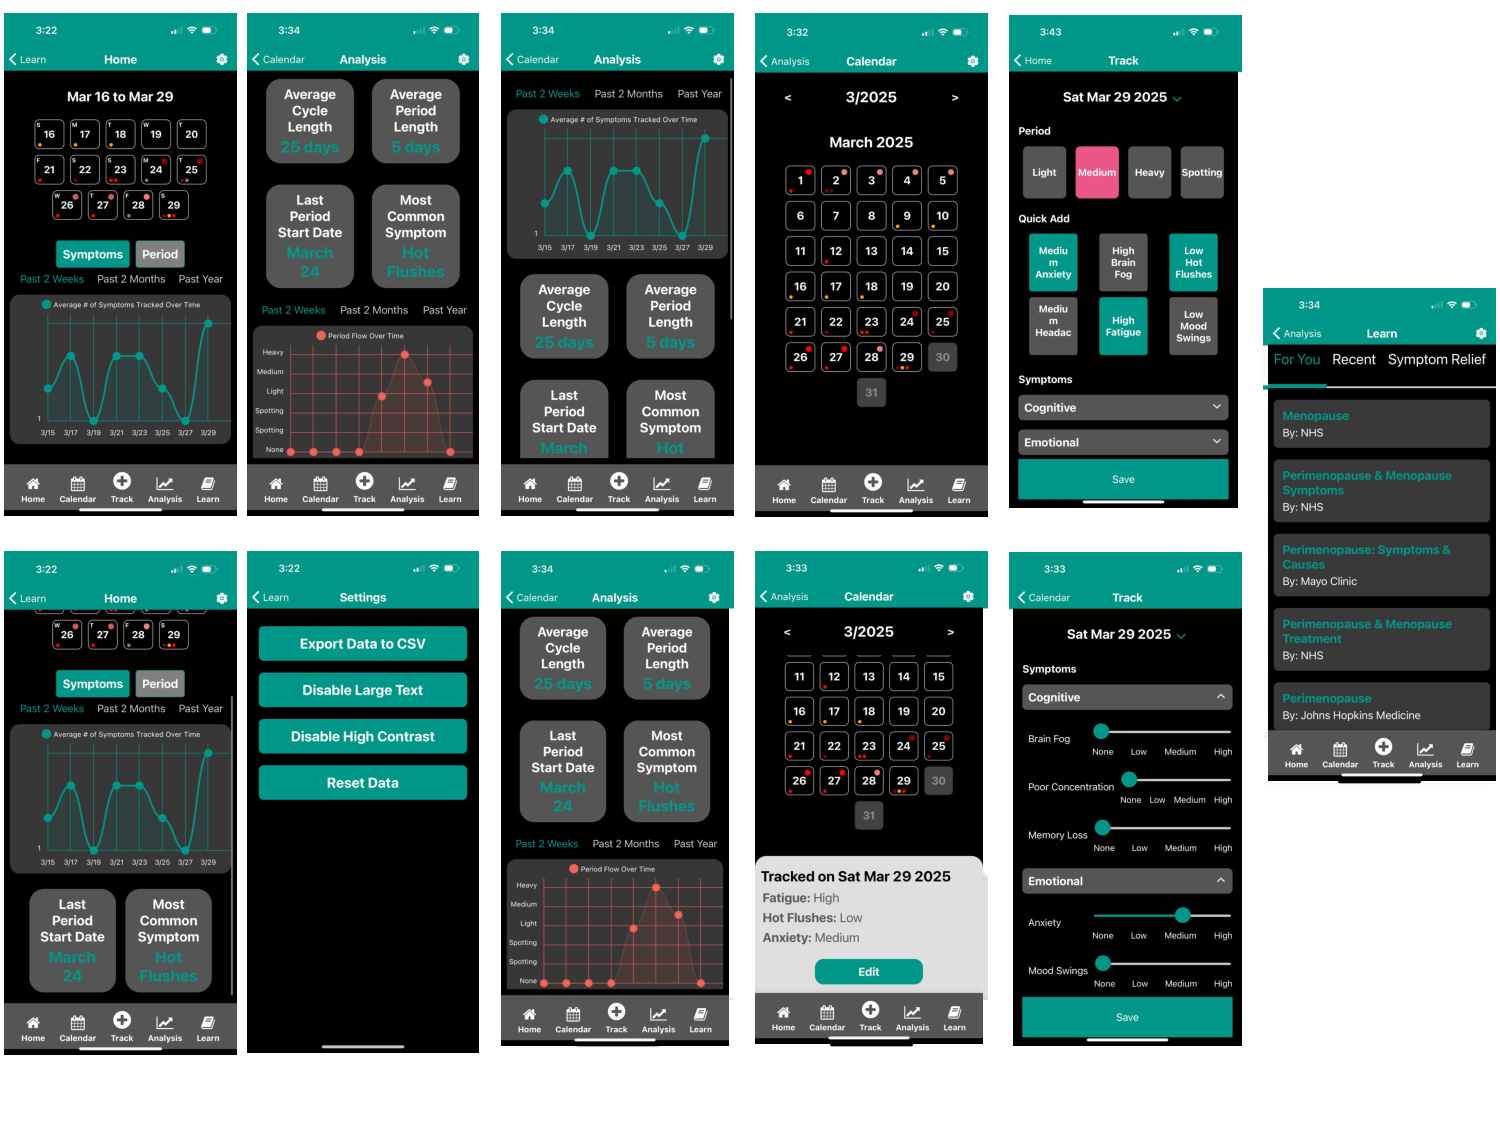
\includegraphics[scale=0.6]{app-Accessible.pdf}
    \caption{Final React Native App Design with high contrast and large text on.}
    \label{figure:app-Accessible}
  \end{center}
\end{figure}

\subsubsection{System Design}
In the interest of protecting user privacy, there is no database and all data is stored on the user's local device. The data that is saved in AsyncStorage on their device is formatted as featured in table\ref{table:user-data}.

\begin{table}[h!!]
    \caption{Structure of User Data Stored in AsyncStorage}
    \label{table:user-data}
    \begin{tabular}{llll}
    \hline
    Anonymous User &        &          &          \\ \hline
                  & Date1  &          &          \\
                  &        & Symptom1 & Severity \\
                  &        & Symptom2 & Severity \\
                  & Date2  &          &          \\
                  &        & Symptom1 & Severity \\
                  &        & Symptom2 & Severity \\
                  & Date n &          &          \\
                  &        & Symptom1 & Severity \\
                  &        & Symptom2 & Severity \\ \hline
  \end{tabular}
\end{table}
